\label{chapter:resultados}

O presente capítulo consiste em apresentar o planejamento, execução, e  análise dos resultados referente ao método proposto. Assim,  visando avaliar de forma experimental o sistema computacional desenvolvido a partir do método proposto, denominado de INEXT, para identificação e localização de objeto em edifícios utilizando RFID.

\section{Planejamento e projeto dos experimentos}

Esta avaliação experimental consiste em avaliar o INEXT, tendo como questões principais a identificação e localização de objetos em ambientes confinados e então o gerenciamento dos objetos. Em virtude disso, foi definida as seguintes questões:

\begin{itemize}

    \item[QP1]: O sistema INEXT consegue identificar e rastrear os objetos em um âmbito confinado?
    \item[QP2]: Quais vantagens o sistema INEXT prove em relação ao gerenciamento dos objetos em edifícios?
    \item[QP3]: O sistema INEXT é capaz de gerar de forma automática o inventário de objetos em um âmbito confinado\todo{Adicionar resposta no texto}?
    
\end{itemize}

\par 
Objetivando responder tais questões de pesquisa, foram utilizados um Arduíno Nano $V3.0$ ATmega168 \todo[color=green]{Adicionar versão} e um computador comunicando-se através da porta serial para simular a segunda sala, pois não disponhamos de duas placas NodeMcu para a comunicação sem fio. Um script na linguagem Python $v 3,7,1$ \todo[color=green]{Versão?} foi adotado para ler os dados da porta serial, criar um objeto JSON e enviar para o servidor, tais código estão disponíveis no repositório deste trabalho (endereço mencionado no \autoref{chapter:metodo} \todo[color=green]{Adicionar seção}) dentro da pasta \texttt{prototype\_arduino}. O computador utilizado possui $4GB$ de memória RAM, processador Intel Core $i5-2500$, HD de $500GB$ e sistema operacional Windows $7$ Professional de $64Bits$. 

Os protótipos dos dispositivos de porta\todo[color=green]{Do que?} podem ser visualizados nas \autoref{fig:prototipo_arduino} e \autoref{fig:prototipo_nodemcu}. A \autoref{fig:prototipo_arduino} mostra o Arduíno Nano juntamente com o leitor RFID RC522 conectados através de \textit{jumpers}, já na \autoref{fig:prototipo_nodemcu} mostra o NodeMcu conectado com o leitor RFID RC522. A prototipação do Arduíno segue abaixo:
\todo[inline,color=green]{Sugiro descrever as figuras mencionadas acima.}


\todo[inline, color=green]{Mover e o esquema de conexão da figura 27 para o método proposto}

\begin{itemize}
    \item 3.3V - conectado ao pino de 3.3v no Arduíno, essa conexão faz a alimentação do leitor RFID;
    \item RST (\textit{Reset})- conectado ao pino 9 do Arduíno;
    \item GND (\textit{graduated neutral density filter}) - conectado ao pino GND do Arduíno;
    \item NC/IRQ (\textit{Interrupt Request})- não utilizado;
    \item MISO (\textit{Master In Slave Out}) - conectado ao pino 12;
    \item MOSI  (\textit{Master Out Slave In}) - conectado ao pino 11;
    \item SCK  (\textit{Serial Clock}) - conectado ao pino 13;
    \item SDA/ SS (\textit{Serial Data Line/ Select Slave}) - conectado ao pino 10.
\end{itemize}    

\begin{comment}
\begin{figure}[H]
              \caption{\label{fig:esq_conexoes_arduino}{Esquema de Conexões Arduíno Nano}}
              \centering
              \includegraphics[width=1\textwidth]{Figuras/esquema_de_conexoes1.PNG}
              \legend{Fonte: Própria}
\end{figure}
\end{comment}

\begin{figure}[H]
              \caption{\label{fig:prototipo_arduino}{Protótipo Arduíno Nano}}
              \centering
              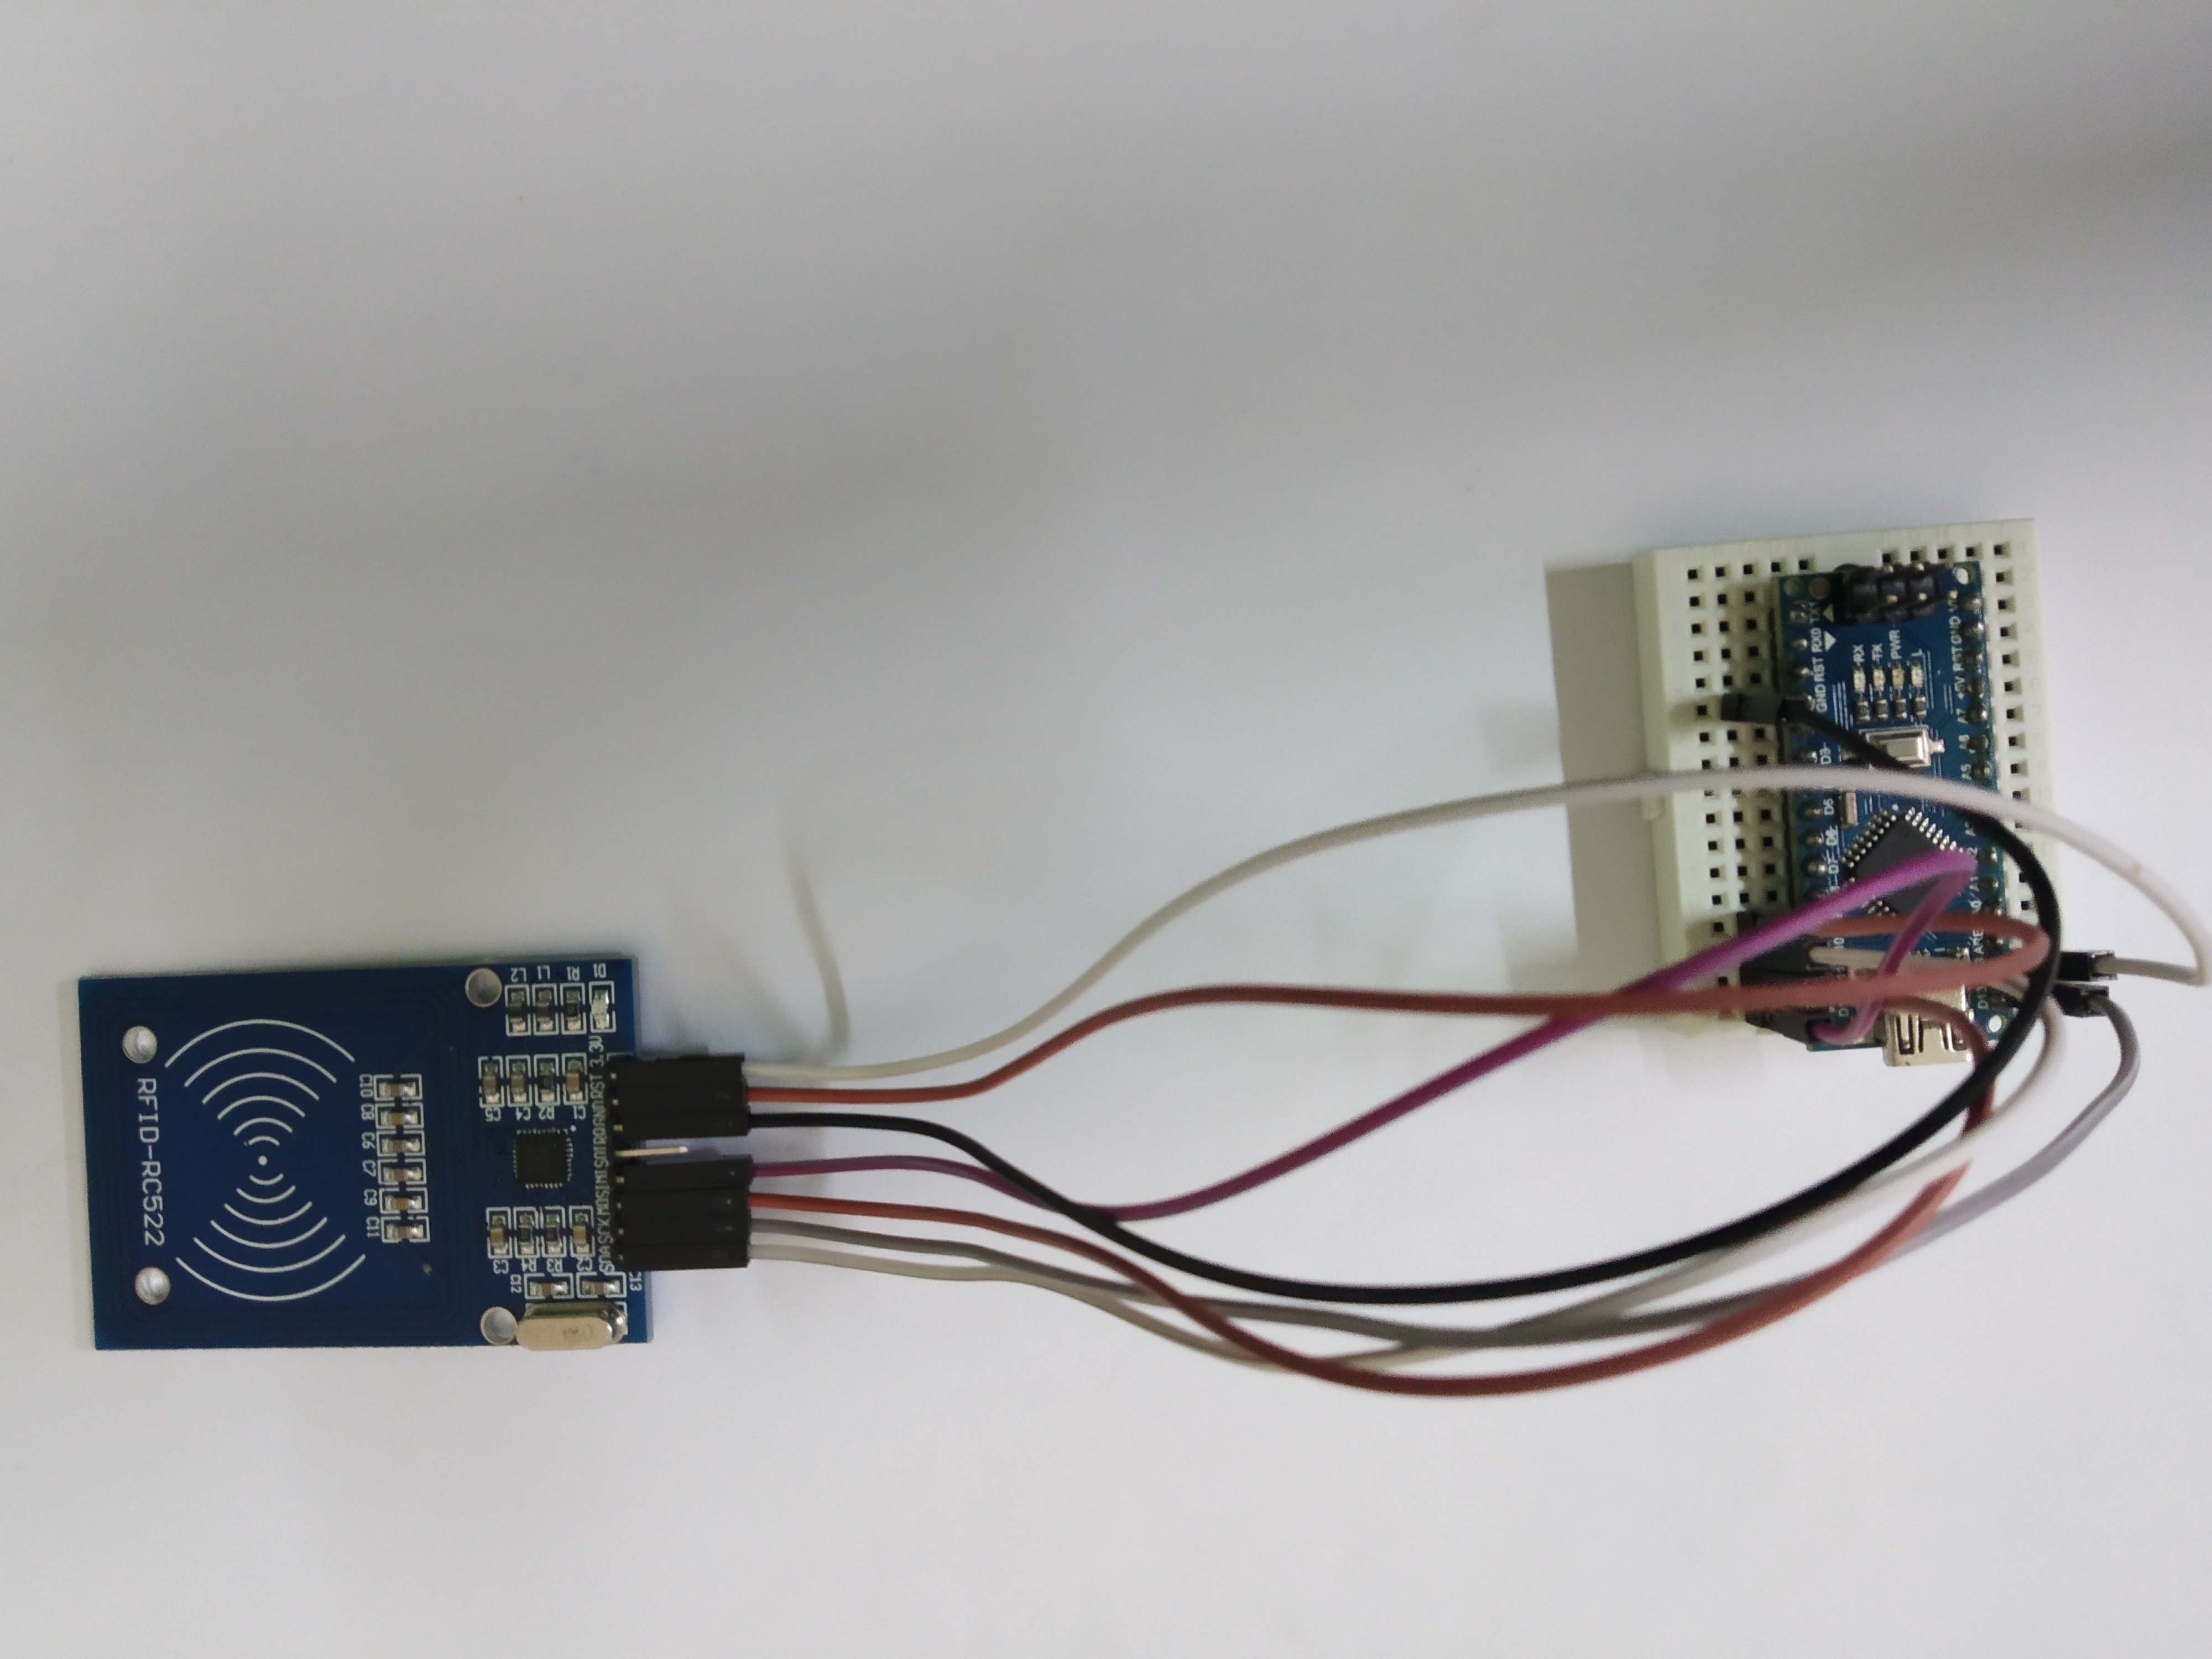
\includegraphics[width=0.7\textwidth]{Figuras/prototype_arduino.png}            \legend{Fonte: Própria}
\end{figure}\begin{figure}[H]
              \caption{\label{fig:prototipo_nodemcu}{Protótipo NodeMcu}}
              \centering
              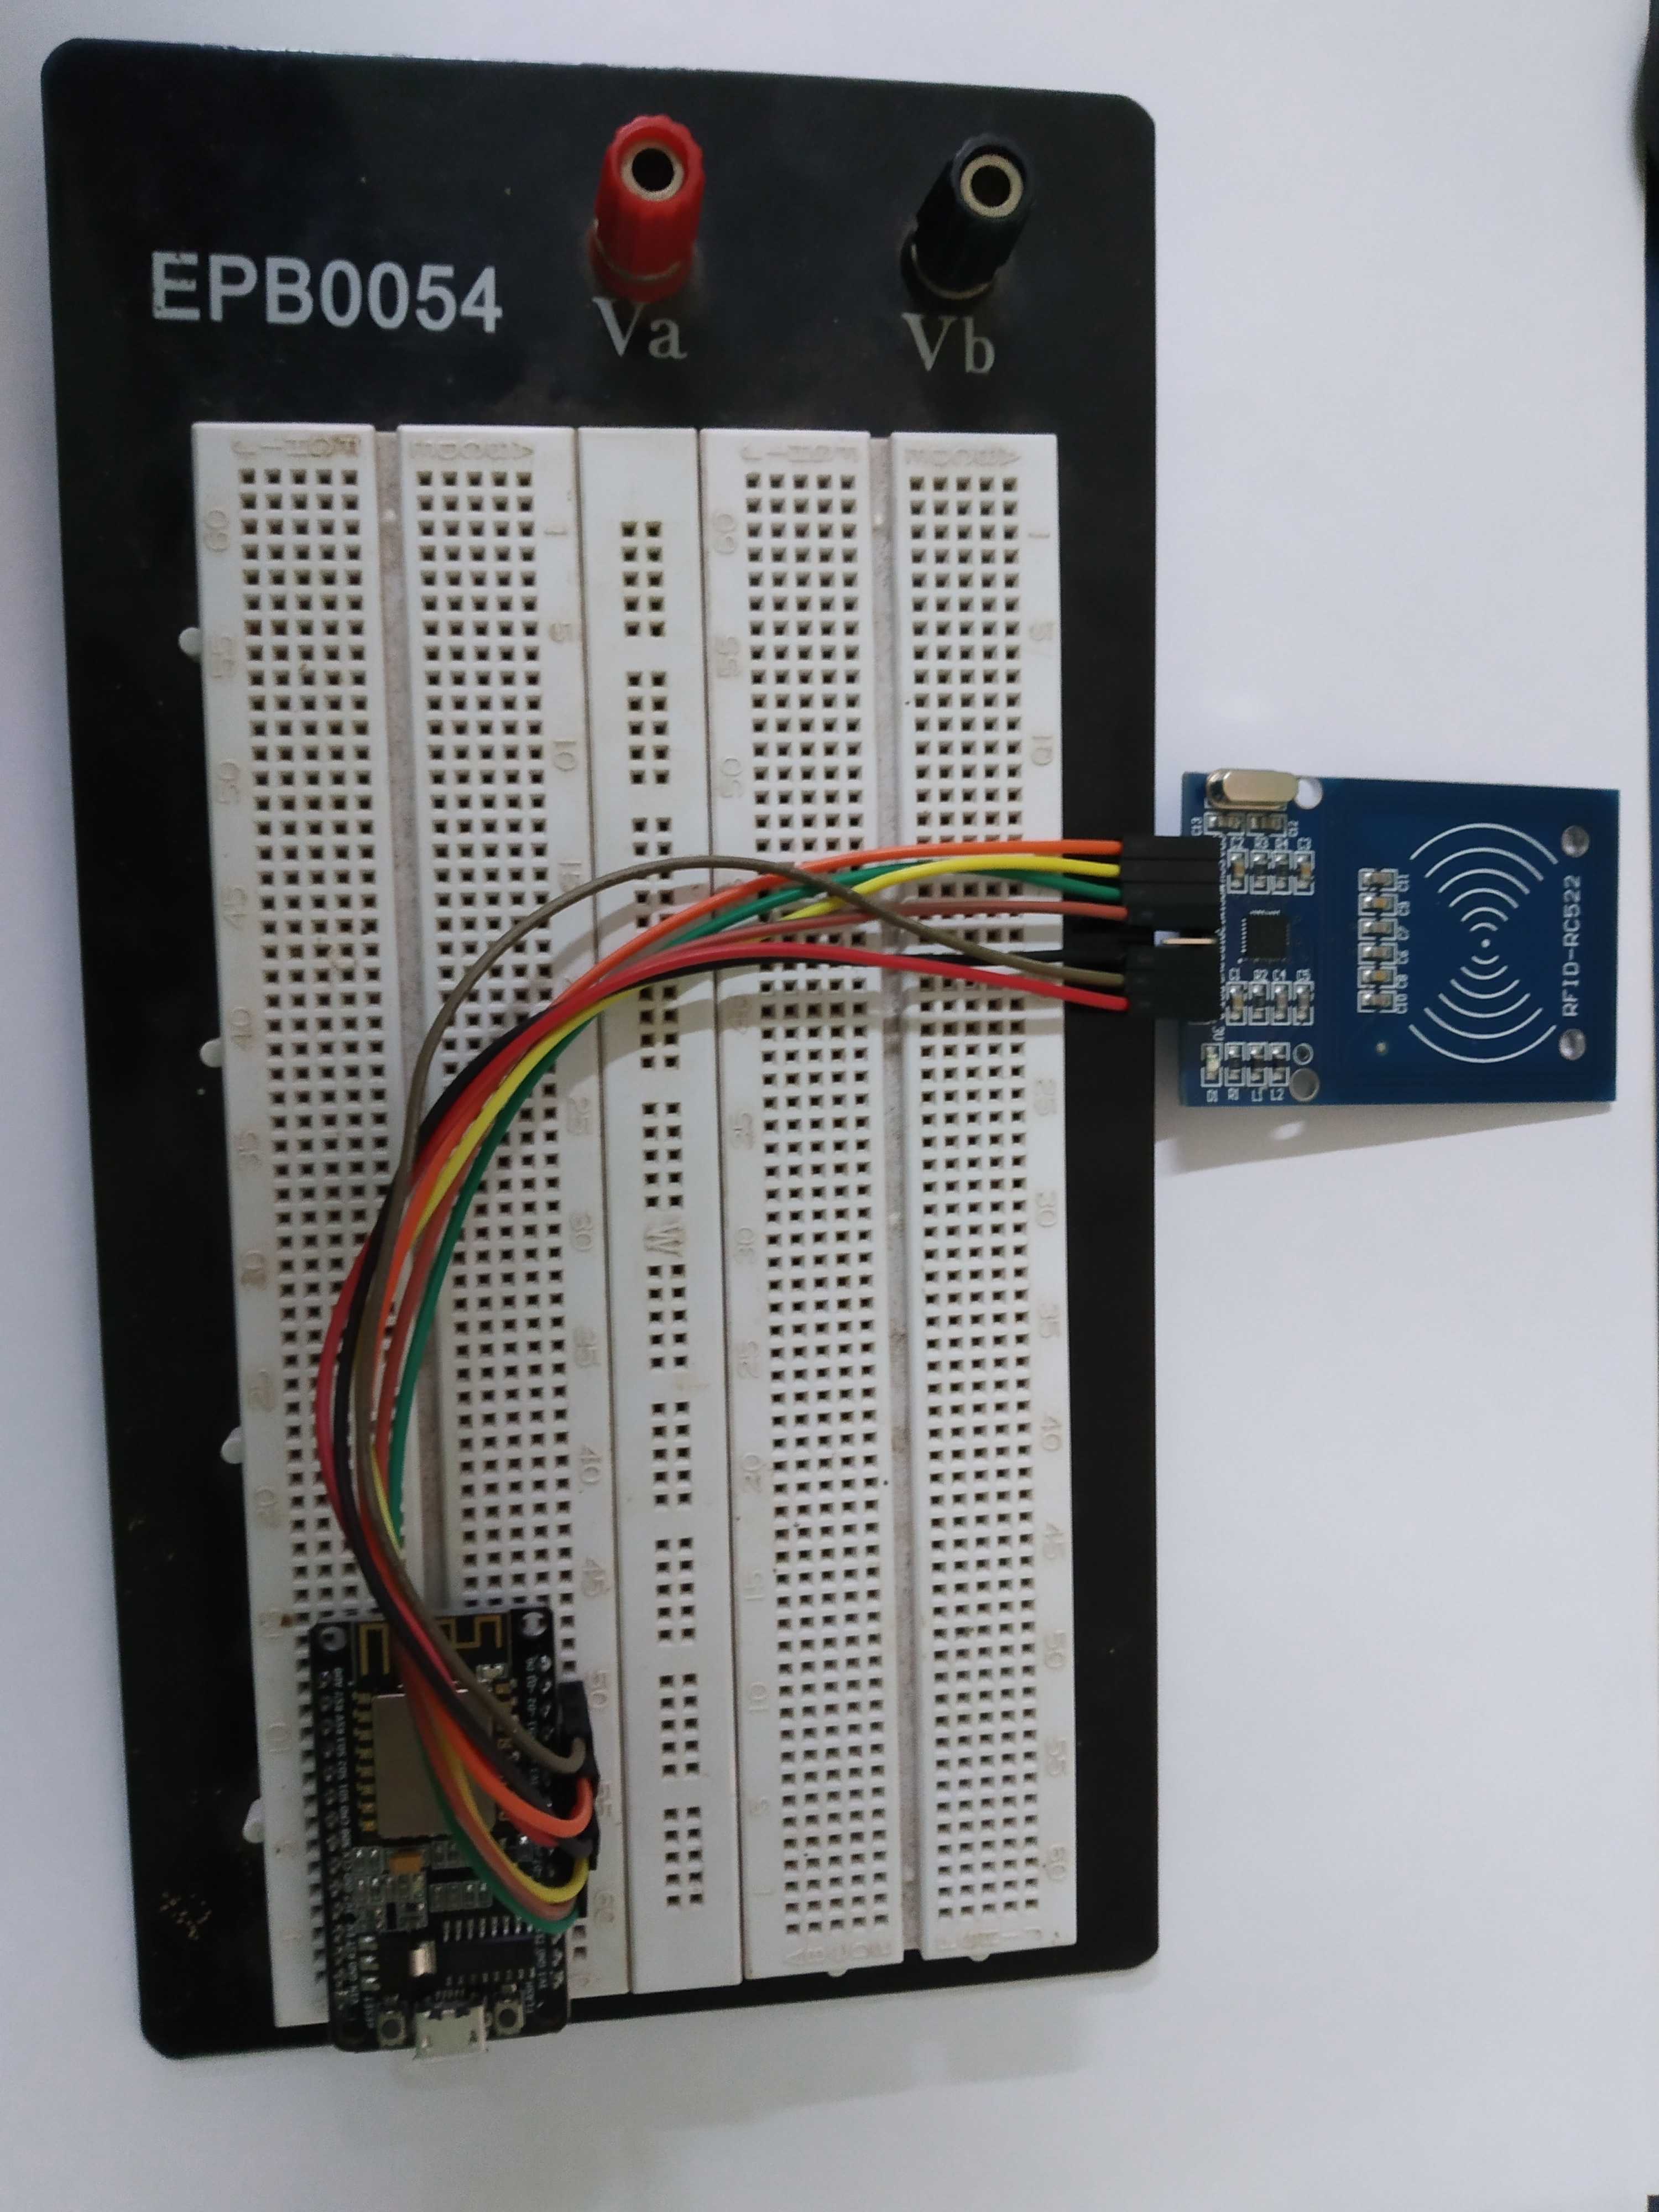
\includegraphics[width=0.5\textwidth]{Figuras/prototype_nodemcu.png}
              \legend{Fonte: Própria}
\end{figure}


\par
Para a simulação do servidor, foi utilizado um notebook com $6GB$ de memória RAM, processador Intel Core $i5-4200$, HD de $750GB$, placa de video GeForce $720M$ de $2GB$ de memória dedicada e sistema operacional Windows $10$ Home Single Language. A rede LAN utilizada foi criada através de um roteador \textit{TP-LINK} modelo $TL-WR720N$. Também foram utilizadas quatro etiquetas RFID passivas, cada uma dessas etiquetas representa um objeto diferente para a simulação.

\todo[color=green,inline]{Sugiro descrever cada um dos cenários propostos na avaliação para responder as questões de pesquisa.}
\par
A execução do experimento aconteceu no cenário apresentado na \autoref{fig:cenario}, foi simulado duas salas e quatro objetos rastreáveis em um edifício. Visando responder as questões foram executados os seguintes testes: (1) localização e identificação dos objetos, no intuído de obter respostas para a primeira pergunta, (2) criação de restrição de objeto afim de verificar se as notificações ao violar restrição são uma forma de se ter melhor gerenciamento dos objetos e (3) levantamento de todos os objetos e as salas que eles estão \todo[color=green]{Mover este texto para seção anterior, e ampliar a descrição focando as questões de pesquisa}.

\begin{figure}[H]
              \caption{\label{fig:cenario}{Cenário de simulação}}
              \centering
              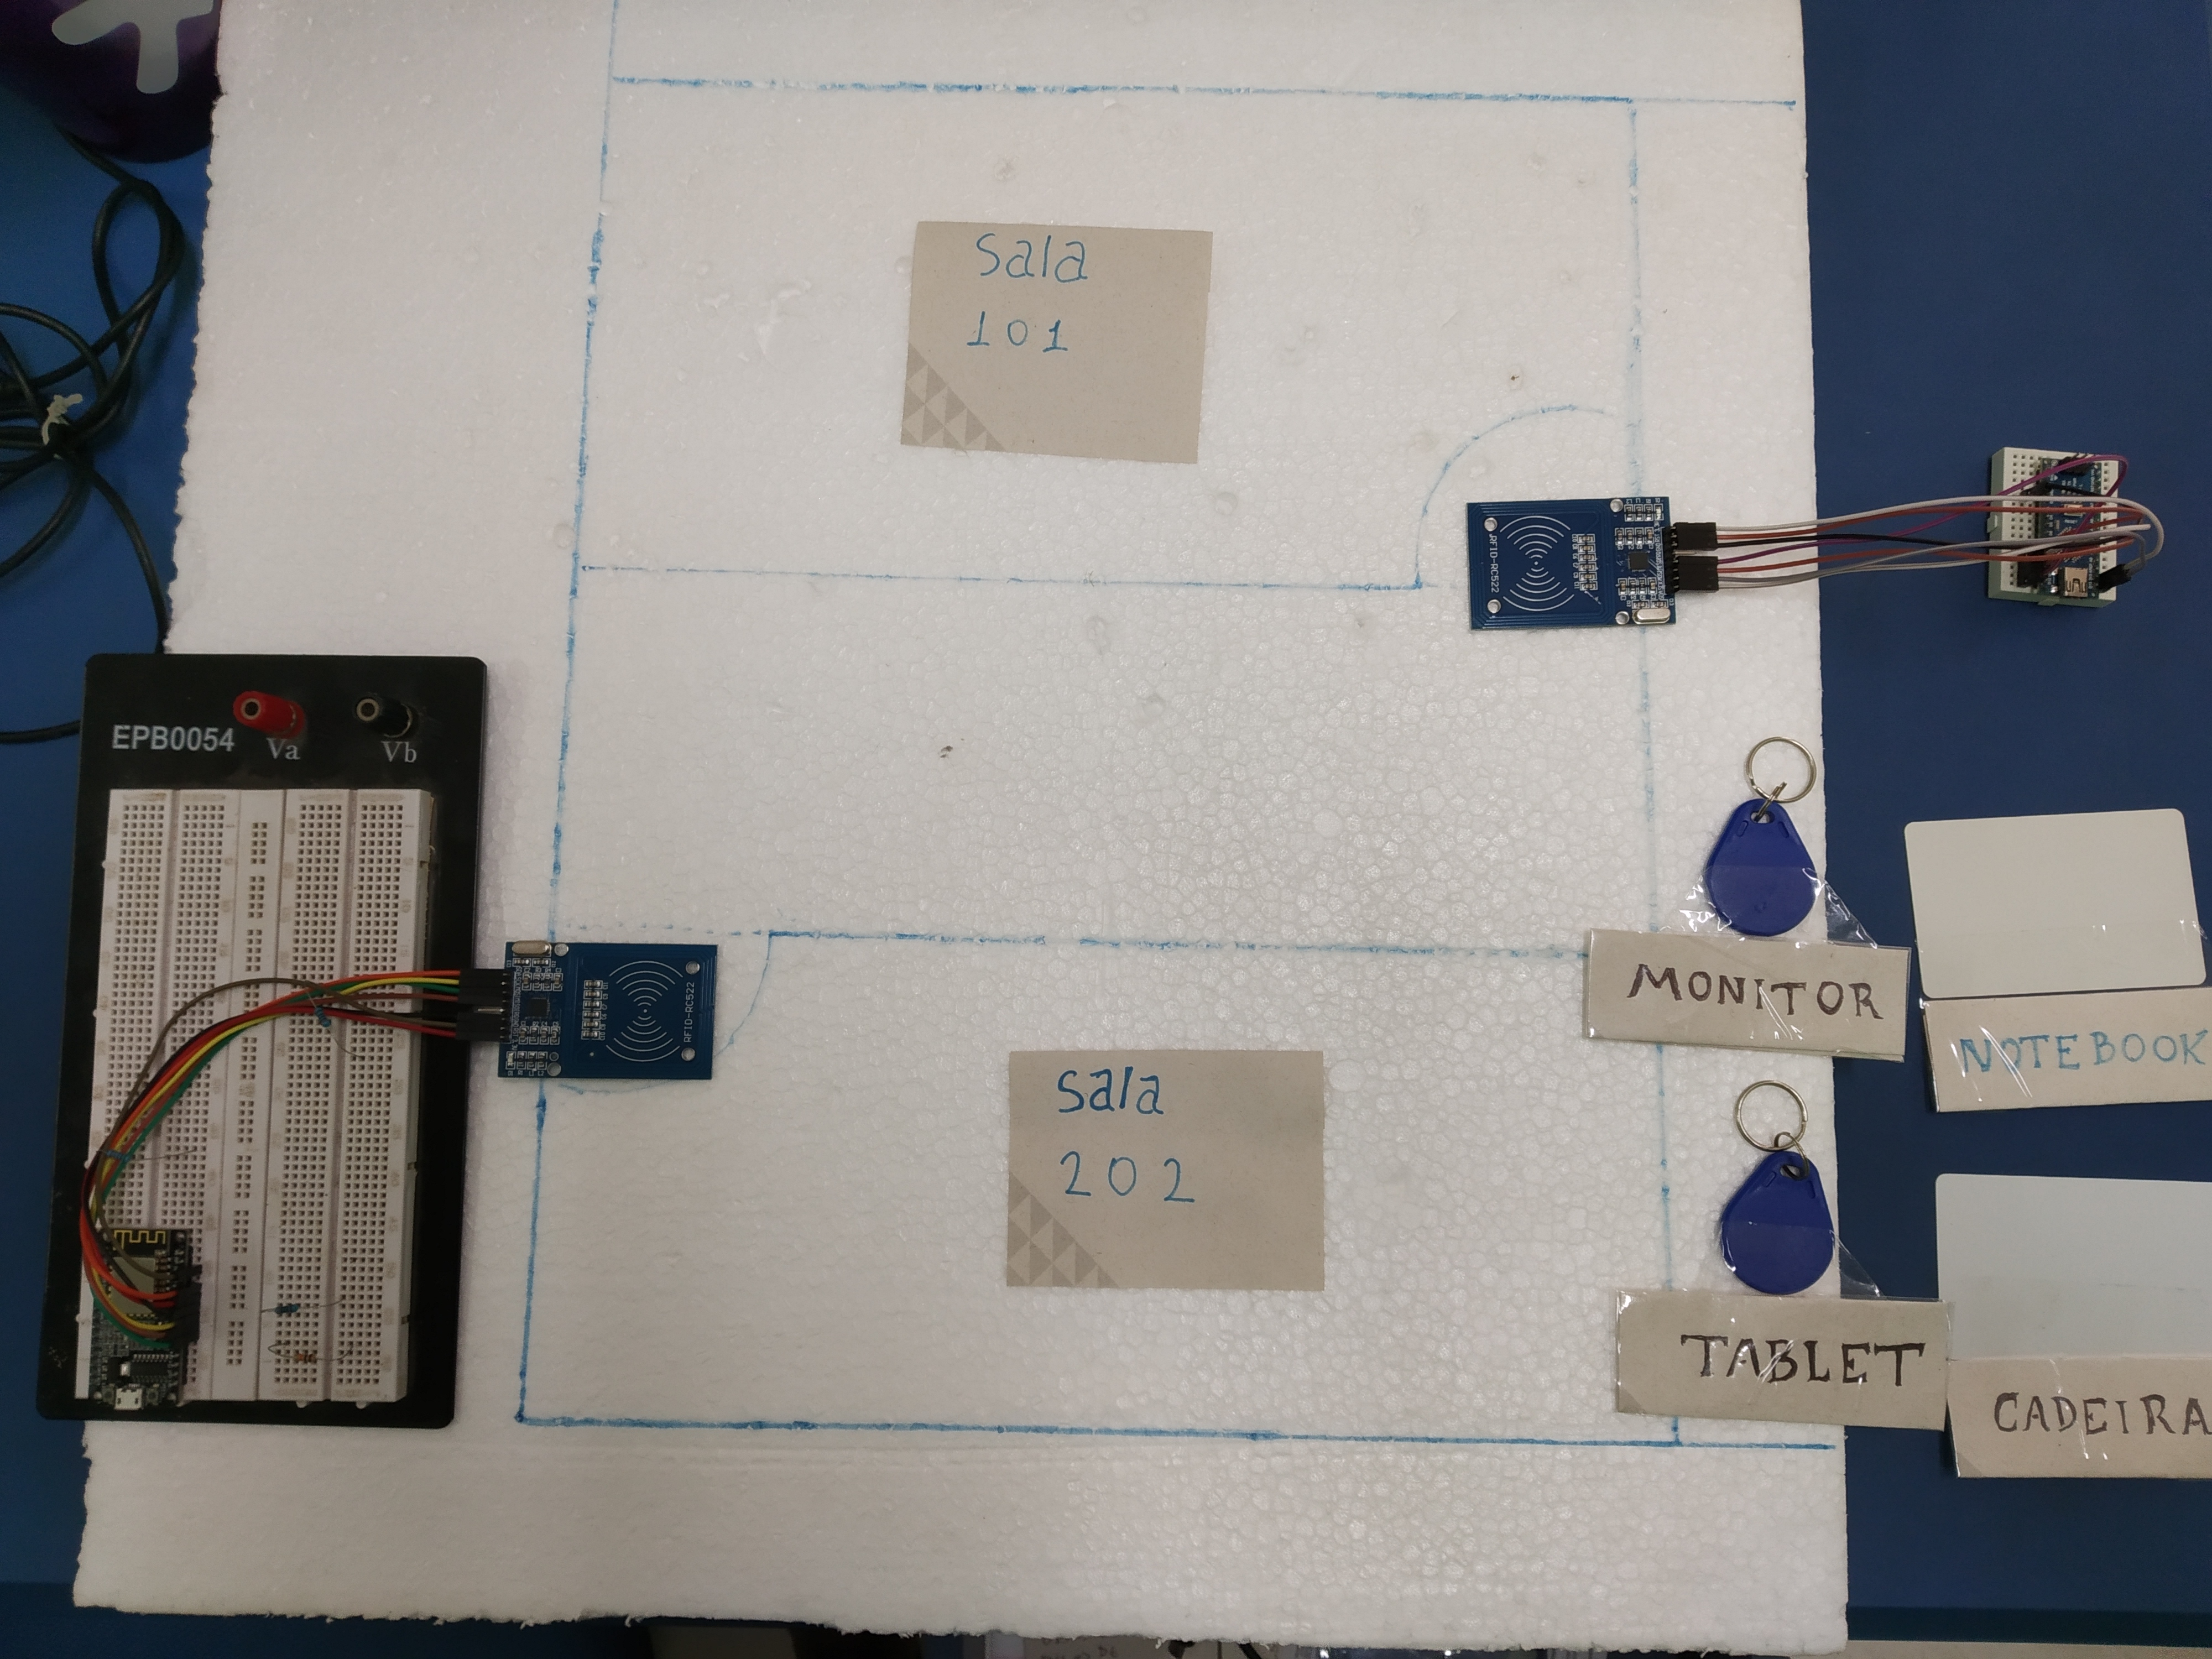
\includegraphics[width=1\textwidth]{Figuras/cenario.png}
              \legend{Fonte: Própria}
\end{figure}
\section{Execução dos experimentos e Análise dos Resultados}

\todo[inline]{A partir daqui você deve descrever os resultados de forma detalhada e respondendo as questões de pesquisa}
 
 Visando responder as questões do planejamento, iniciamos os testes do cenário (1) cadastrando as quatro etiquetas no sistema e identificando-as cada uma como um objeto diferente, duas etiquetas foram lidas pelo dispositivo de porta da sala $101$ e as outras duas foram lidas pelo dispositivo de porta da sala $202$, o \textit{pipiline} do processo pode ser visualizado na \autoref{fig:piptransicao} de A até D, esse processo foi repetido mais três vezes e o resultado final desse processo com as quatro etiquetas esta na ultima figura.

\begin{figure}[ht]
        \centering\caption{Identificação dos objeto}
        \label{fig:piptransicao}
       \subfloat[A\label{fig:execution1a}]{
            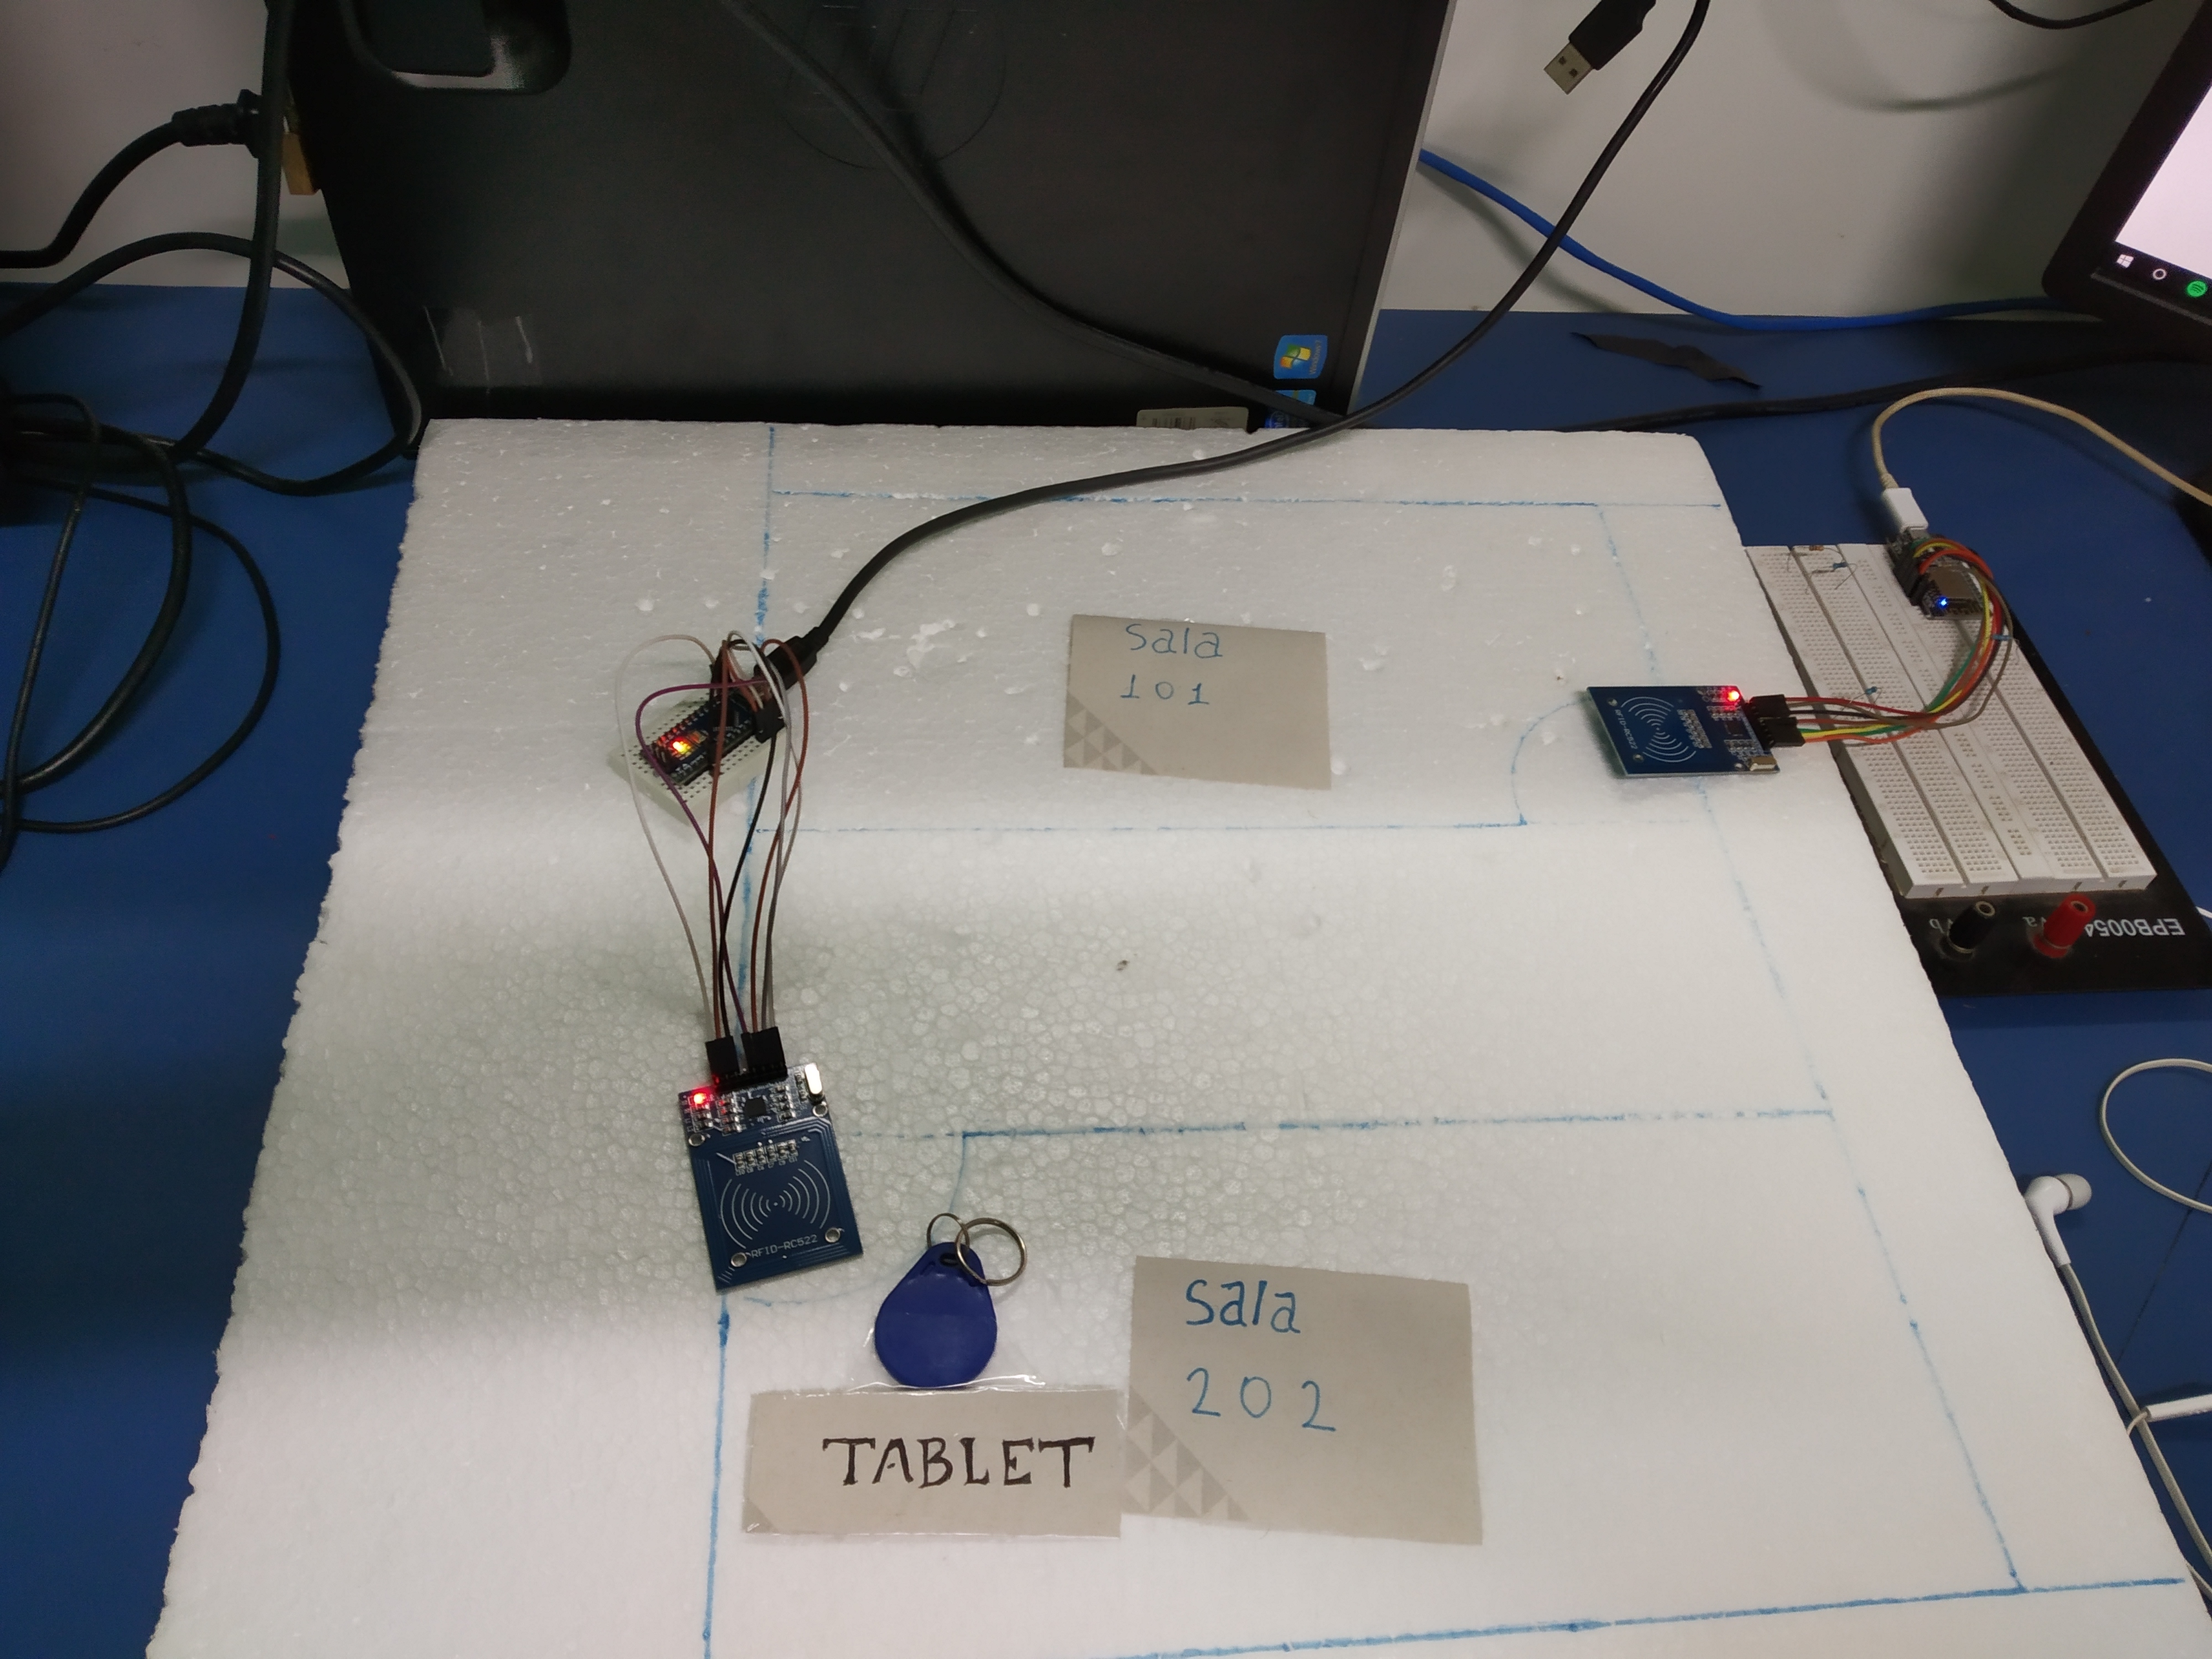
\includegraphics[width=0.4\textwidth]{Figuras/execucao1a.PNG}}
         \hspace{0.5cm}
       \subfloat[B\label{fig:execution1b}]{
            \includegraphics[width=0.4\textwidth]{Figuras/execucao1.PNG}}
             \hspace{0.5cm}
       \subfloat[C\label{fig:execution1c}]{
            \includegraphics[width=0.4\textwidth]{Figuras/execucao1br.PNG}}
        \hspace{0.5cm}
       \subfloat[D\label{fig:execution1d}]{
            \includegraphics[width=0.4\textwidth]{Figuras/execucao1c.PNG}}
             \hspace{0.5cm}
       \subfloat[E\label{fig:execution1f}]{
             \includegraphics[width=0.4\textwidth]{Figuras/execution1F.PNG}}
              \hspace{0.5cm}
      \legend{Fonte: Própria}
\end{figure}

\par
Ainda realizando teste no cenário (1), executamos o processo de transição dos objetos onde uma etiqueta é lida quando sai da sala e quando entra na outra sala, esse \textit{pipiline} pode ser visto na \autoref{fig:piptransicao} de \texttt{A} até \texttt{E}. Foram executadas transições para todos objetos onde os objetos que estavam na sala 101 ficaram na sala 202 e os da sala 202 foram para a sala 101.

\begin{figure}[ht]
        \centering\caption{Transição de objeto}
        \label{fig:piptransicao}
       \subfloat[A\label{fig:execution2a}]{
            \includegraphics[width=0.4\textwidth]{Figuras/execution2a.png}}
         \hspace{0.5cm}
       \subfloat[B\label{fig:execution2b}]{
            \includegraphics[width=0.4\textwidth]{Figuras/execution2c.png}}
             \hspace{0.5cm}
       \subfloat[C\label{fig:execution2c}]{
            \includegraphics[width=0.4\textwidth]{Figuras/execution2b.png}}
        \hspace{0.5cm}
       \subfloat[D\label{fig:execution2d}]{
            \includegraphics[width=0.4\textwidth]{Figuras/execution2d.png}}
             \hspace{0.5cm}
       \subfloat[E\label{fig:execution2c}]{
             \includegraphics[width=0.4\textwidth]{Figuras/execution2e.png}}
              \hspace{0.5cm}
        
      \legend{Fonte: Própria}
\end{figure}

\par
No cenário (2), foram criados dois usuário na tela de quem notificar para receber as notificações via email, para isso foi utilizado o email's do próprio autor, em seguida foi criado restrição para cada objeto. Na tela principal cada objeto possui uma opção para editar ao seu lado, foi editado um objeto por vez colocando no campo restrição o mesmo nome que ele possuía no campo de \texttt{localização(sala)}. O cadastro dos usuários e a edição dos objetos pode ser visualizado no \textit{pipiline} da \autoref{fig:cadRest}.

\begin{figure}[ht]
        \centering\caption{Cadastro de usuários e Criação de Restrições de objeto}
        \label{fig:cadRest}
       \subfloat[A\label{fig:execution3a}]{
            \includegraphics[width=0.4\textwidth]{Figuras/execution3a.png}}
         \hspace{0.5cm}
       \subfloat[B\label{fig:execution3b}]{
            \includegraphics[width=0.4\textwidth]{Figuras/execution3b.png}}
             \hspace{0.5cm}
       \subfloat[C\label{fig:execution3c}]{
            \includegraphics[width=0.4\textwidth]{Figuras/execution3c.png}}
        \hspace{0.5cm}
       \subfloat[D\label{fig:execution3d}]{
            \includegraphics[width=0.4\textwidth]{Figuras/execution3d.png}}
             \hspace{0.5cm}
       \subfloat[E\label{fig:execution3e}]{
             \includegraphics[width=0.4\textwidth]{Figuras/execution3e.png}}
              \hspace{0.5cm}
      \legend{Fonte: Própria}
\end{figure}
\par
Ainda no cenário (2), foi realizado processo de transição com os objetos afim de verificar se o sistema notifica os usuários através do e-mail e na tela inicial, o \textit{pipiline} da execução esta na \autoref{fig:transicaoeRest}. Foram realizadas transições para todos os objetos com restrições.

\begin{figure}[ht]
        \centering\caption{Transições com Restrições}
        \label{fig:transicaoeRest}
       \subfloat[A\label{fig:execution4a}]{
            \includegraphics[width=0.4\textwidth]{Figuras/execution4a.png}}
         \hspace{0.5cm}
       \subfloat[B\label{fig:execution4b}]{
            \includegraphics[width=0.4\textwidth]{Figuras/execution4b.png}}
             \hspace{0.5cm}
       \subfloat[C\label{fig:execution4c}]{
            \includegraphics[width=0.4\textwidth]{Figuras/execution4c.png}}
        \hspace{0.5cm}
       \subfloat[D\label{fig:execution4d}]{
            \includegraphics[width=0.4\textwidth]{Figuras/execution4d.png}}
             \hspace{0.5cm}
       \subfloat[E\label{fig:execution4c}]{
             \includegraphics[width=0.4\textwidth]{Figuras/execution4e.png}}
              \hspace{0.5cm}
        \subfloat[E\label{fig:execution4d}]{
             \includegraphics[width=0.4\textwidth]{Figuras/execution4e.png}}
              \hspace{0.5cm}      
        \subfloat[E\label{fig:execution4e}]{
             \includegraphics[width=0.4\textwidth]{Figuras/execution4e.png}}
              \hspace{0.5cm}
      \legend{Fonte: Própria}
\end{figure}
No cenário (3) é o levantamento de todos objetos cadastrados no sistema com suas respectivas salas, primeiramente é necessário ir até a tela \texttt{Ger. de Salas} para verificar as salas cadastradas no sistema e em seguida ir para a tela \texttt{Inventário}. O \textit{pipiline} das duas execuções desse processo está na \autoref{fig:invent}.

\begin{figure}[ht]
        \centering\caption{Inventário}
        \label{fig:invent}
       \subfloat[A\label{fig:execution5a}]{
            \includegraphics[width=0.4\textwidth]{Figuras/execution5a.png}}
         \hspace{0.5cm}
       \subfloat[B\label{fig:execution5b}]{
            \includegraphics[width=0.4\textwidth]{Figuras/execution5b.png}}
             \hspace{0.5cm}
       \subfloat[C\label{fig:execution5c}]{
            \includegraphics[width=0.4\textwidth]{Figuras/execution5c.png}}
        \hspace{0.5cm}
       \subfloat[D\label{fig:execution5d}]{
            \includegraphics[width=0.4\textwidth]{Figuras/execution5d.png}}
             \hspace{0.5cm}
       \subfloat[E\label{fig:execution5c}]{
             \includegraphics[width=0.4\textwidth]{Figuras/execution5e.png}}
              \hspace{0.5cm}
        
      \legend{Fonte: Própria}
\end{figure}
\subsection{Resultados}

Após a execução dos testes, foram obtidos os resultados apresentados na \autoref{tab:resultados}, onde cada linha representa um cenário de execução com os números de execuções, número de execuções que funcionaram, números de execuções que funcionaram mas por alguma questão não funcionou perfeitamente, e as que falharam.

\todo[inline, color=green]{Adicionar figuras com a execução de cada cenário, discutindo as ações em termos de vantagens e desvantagens da execução do sistema}
\todo[inline]{Seria bom relacionar a execução dos cenários as tecnologias usadas no sistema}
\begin{table}[htbp]
  \caption{Resultados}
  \label{tab:resultados}
  \begin{tabularx}{\textwidth}{|X|c|c|c|c|c|}
     \hline
    & \textbf{N$^{\circ}$ de execuções} & \textbf{Funcionou } & \textbf{Parcialmente} & \textbf{Falhou} \\
    \hline
    Cenário 1 & 4 & 3 & & 1\\
    \hline
    Cenário 2 & 4 & 4 &  &\\
    \hline
     Cenário 3 & 2 & 1 & 1 &\\
    \hline

  \end{tabularx}
\end{table}

\par
O INEXT conseguiu localizar objetos em ambientes confinados, porém o sistema não proporciona a posição real do objeto no ambiente, o sistema também foi capaz de identificar os objetos mas essa etapa ainda ocorre de maneira manual necessitando ser realizada por usuários. Durante os teste houve uma execução em que os \textit{script} em Python travou e não enviou o JSON gerado para o servidor e ocasionando a perda da localização de um objeto, essa é a execução cujo esta na tabela que falhou.

\par
O sistema proporcionou uma boa forma de gerenciar os objetos de forma que conseguiu informar os usuários sobre as violação de restrições através do e-mail e também da tela principal do sistema, gerando uma nova tabela com os objetos que violaram suas restrições.

\par
Durante a primeira tentativa de gerar o inventário dos objetos cadastrados no sistema, houve repetição de dados justamente porque foram criadas salas repetidas no banco de dados, para solucionara esse problema foi necessário ir até a tela \texttt{Ger. de Salas} e remover as salas repetidas, dessa forma a geração do inventário funcionou sem a repetição dos objetos e salas.

\par

